\documentclass[a4paper]{article}
%~~~~~~~~~~~~~~~~~~~~~~~~~~~~~Packages~~~~~~~~~~~~~~~~~~~~~~~~~~~~%
\usepackage[english]{babel}
\usepackage[utf8x]{inputenc}
\usepackage{booktabs}
\usepackage{tabu}
\usepackage{cancel}
%% Sets page size and margins
\usepackage[a4paper,top=2cm,bottom=2cm,left=2cm,right=2cm,marginparwidth=1.75cm]{geometry}
\usepackage{mymacros}
\usepackage{amsmath}
\usepackage{enumitem}
\usepackage{listings}
\usepackage{relsize}
\usepackage{graphicx}
\usepackage{subcaption}
%\usepackage{apacite}
\usepackage{pgfplots}
\usepackage{comment}
\usepackage{lmodern,textcomp}%For € symbol
\usepackage[colorinlistoftodos]{todonotes}
\usepackage[colorlinks=true, allcolors=blue]{hyperref}

%~~~~~~~~~~~~~~~~~~~~~~~~~~~~~Commands~~~~~~~~~~~~~~~~~~~~~~~~~~~~%

\renewcommand{\abstractname}{Summary}

%~~~~~~~~~~~~~~~~~~~~~~~~~~~~~pgfPlots~~~~~~~~~~~~~~~~~~~~~~~~~~~~%

\pgfplotsset{compat=1.8}
\usepgfplotslibrary{statistics}
%%%%%%%%%%%%%%%%%%%%%%%%%%%%%%%%%%%%%%%%%%%%%%%%%%%%%%%%%%%%%%%%%%%%

\begin{document}

\begin{titlepage}
\begin{center}
\vspace{3cm}

\Large

\vspace{2cm}

  
\includegraphics[scale=0.3]{imgs/Cherubino.jpg}

\vspace{2.5cm}

{\Huge \sc Data mining project report}

\vspace{1cm}

Group 1:
\vspace{1cm}


Maddalena Amendola

\vspace{1cm}

Daniele Gadler

\vspace{1cm}

Riccardo Manetti

\vspace{1cm}

Gemma Martini

\vfill

\today

\end{center}
\end{titlepage}

%%%%%%%%%%%%~~~~~~~~~~~~~~~~~~~~~~~~~~~~~~~~~~~~~~~~~~~%%%%%%%%%%%%

\tableofcontents
\newpage

%%%%%%%%%%%%%%~~~~~~~~~~~~~~~~~~~~~~~~~~~~~~~~~~~~~~~~~~~%%%%%%%%%%
%\author{  Group 1\\ Amendola Maddalena, Daniele Gadler, Gemma Martini, Riccardo Manetti  \\Department of Computer Science, University of Pisa \\ \date{ 1nd Semester of Academic Year 2018--2019}

%\begin{abstract}
 %  This is the abstract text
%\end{abstract}


\section{Data Understanding}

This part contains a first analysis of the data contained in the Taiwan credit card dataset. The collected data takes into account users movements on their bank accounts from April 2005 to September 2005.



\subsection{Outliers' Identification}
These boxplots are created with Python and give us the chance to understand the shape of the given dataset, in order to find out possible outlayers, which may give ah hint on the many characteristics of the data.
                         %~~~~~~~~~%
\subsubsection{Age}
From this plot we can observe that age has some values below $0$. We can assume that the values allowed for this field are strictly positive.

\addplot{0.7}{../Code/Gemma/boxplots/age.png}{Caption}{fig:age}

\begin{center}
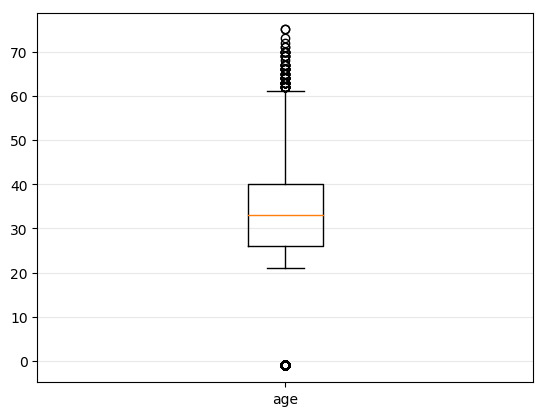
\includegraphics[width=0.9\textwidth]{../Code/Gemma/boxplots/age.png}
\end{center}
                         %~~~~~~~~~%
\subsubsection{Limit}
Since the dataset takes into account Taiwanese dollars ($\sim 0,028$ €) plotting the boxplot in terms of multiples of the average Taiwanese income (NTD $49989$, about USD $1700$) is more informative.
\begin{center}
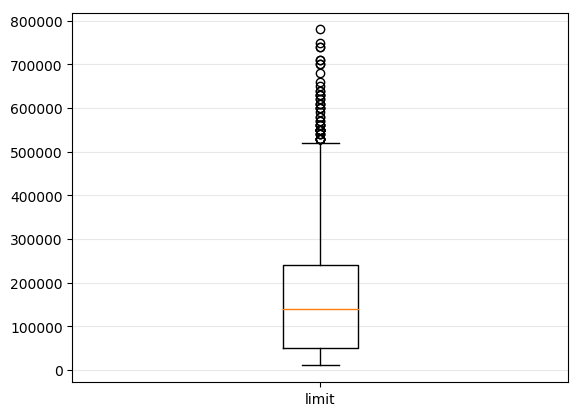
\includegraphics[width=0.48\textwidth]{../Code/Gemma/boxplots/limit.png}
\todo{Daniele: plot limitS.png is missing}

%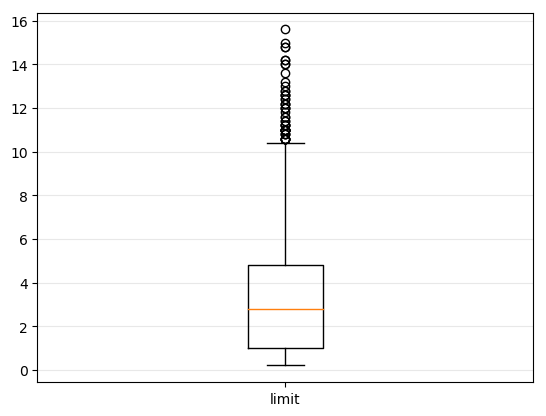
\includegraphics[width=0.45\textwidth]{../Code/Gemma/boxplots/limitS.png}
\end{center}
From this plot we may observe that on average the limit of the credit card plafond is $2.5$ times the average income.
                         %~~~~~~~~~%
\subsubsection{Billing amount}
This values represents the balance of the bank account during the previous billing cycle.
I can't understand what all these outlayers mean!!!
\todo{I can't understand}
\begin{center}
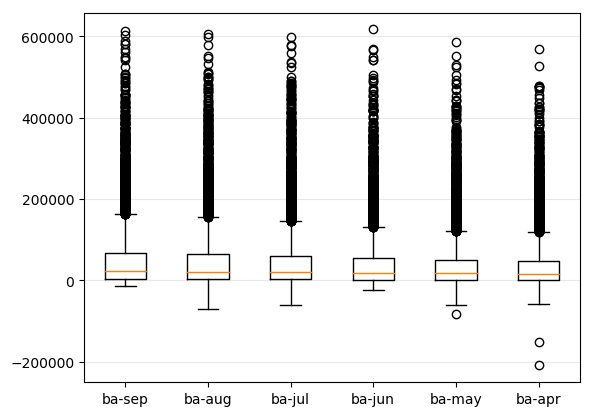
\includegraphics[width=0.9\textwidth]{../Code/Gemma/boxplots/ba.png}
\end{center}
                         %~~~~~~~~~%
\subsubsection{Amount of previous payments}
This values tell us how much the user spent each month in the past 6 months, on a monthly basis.
\todo{Non capisco\\:-C}
\begin{center}
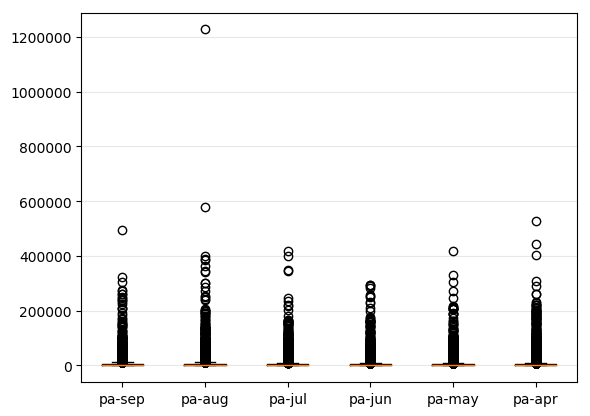
\includegraphics[width=0.9\textwidth]{../Code/Gemma/boxplots/pa.png}
\end{center}
                         %~~~~~~~~~%
\subsubsection{Payment status}
This columns of the database contain the history of payments, more precisely:
\begin{description}
  \item[\sc Payed in time]$\rightarrow$ value $-1$

  \item[\sc Paid one month later]$\rightarrow$ value $1$

  \item[\sc Paid two months later]$\rightarrow$ value $2$

  \item[\sc Paid three months later]$\rightarrow$ value $3$

  \item[\sc Paid four months later]$\rightarrow$ value $4$

  \item[\sc Paid five months later]$\rightarrow$ value $5$

  \item[\sc Paid six months later]$\rightarrow$ value $6$

  \item[\sc Paid seven months later]$\rightarrow$ value $7$

  \item[\sc Paid eight months later]$\rightarrow$ value $8$

  \item[\sc Paid nine months later or more]$\rightarrow$ value $9$
\end{description}
\begin{center}
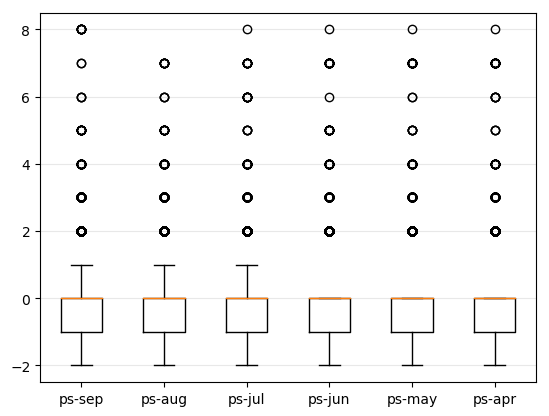
\includegraphics[width=0.9\textwidth]{../Code/Gemma/boxplots/ps.png}
\end{center}
\todo{Direi che questo lo togliamo\\\ldots???}


\newpage


\subsection{Context-specific Dependencies}

To achieve a deeper insight into the dataset under study, let's first analyze some basic statistics and correlations about the dataset by analyzing some interesting properties of the dataset.

\subsubsection{Customer Balance and Payments over months}


\begin{center}
\begin{figure}

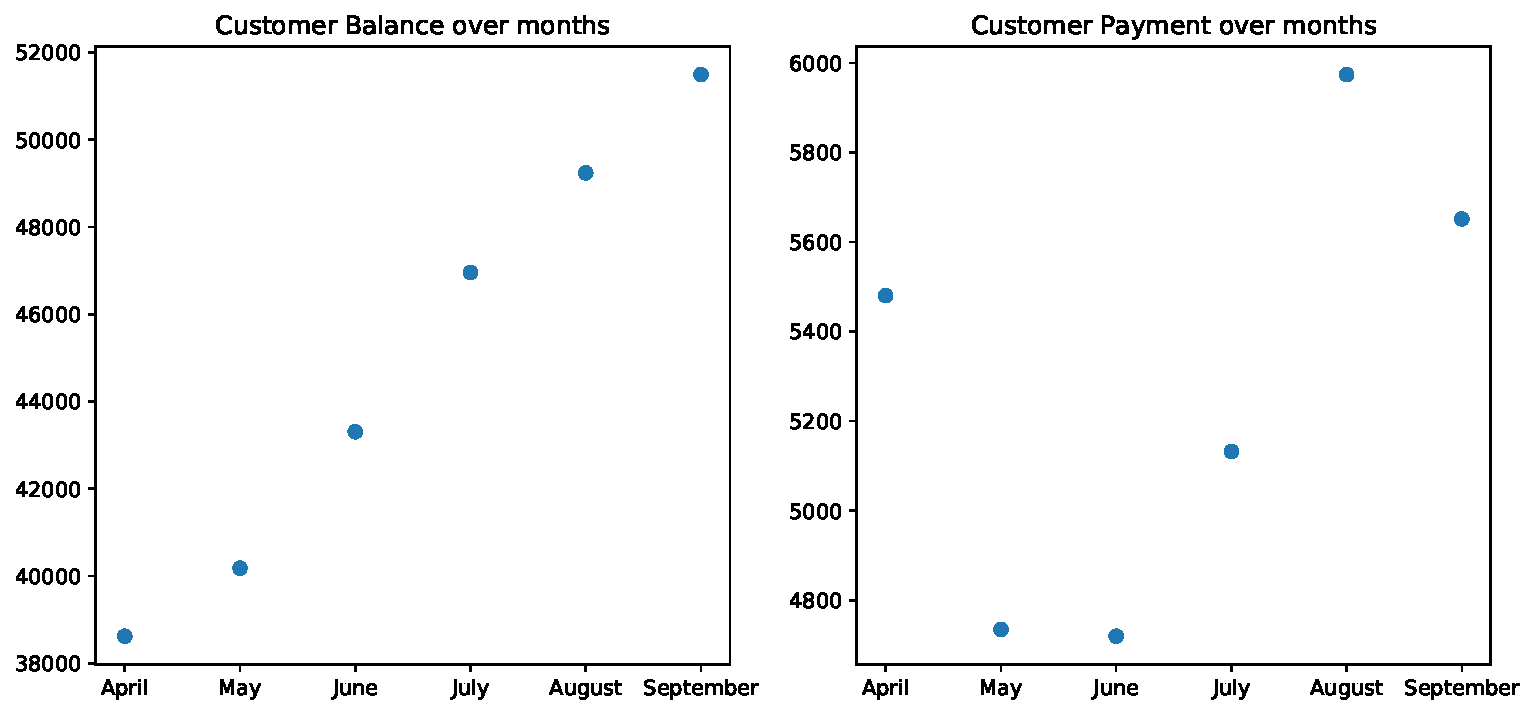
\includegraphics[width=0.9\textwidth]{../Code/Daniele/Plots/average_months.pdf}
\caption{Plot of the average customer balance and payments over the April, May, June, July, August and September months }
\label{average_months}


\end{figure}
\end{center}



\begin{enumerate}

\item{\textbf{Overall Trend}}

As it is expected from a bank account dataset, the customer balance tends to increase over the months. On the other hand, the amount spent by customers is not fixed over time: it is maximum during August and September - because of an increased spending, probably on holidays - and is minimum during May and June, simple working months in Taiwan. 

\textit{Correlation between customer balance and payments}: As the plotted attributes in Figure \label{average_months} seem to be characterized by different growth patterns, the correlation between the average customer balance and the average payment is just $0.355$, and thus does not suggest a strong correlation. 




\item \textbf{Age}

As it is expected, older people generally have a higher balance than young people: also, people in their 60s tend to spend more than young or middle-aged people. 

\begin{center}
\begin{figure}

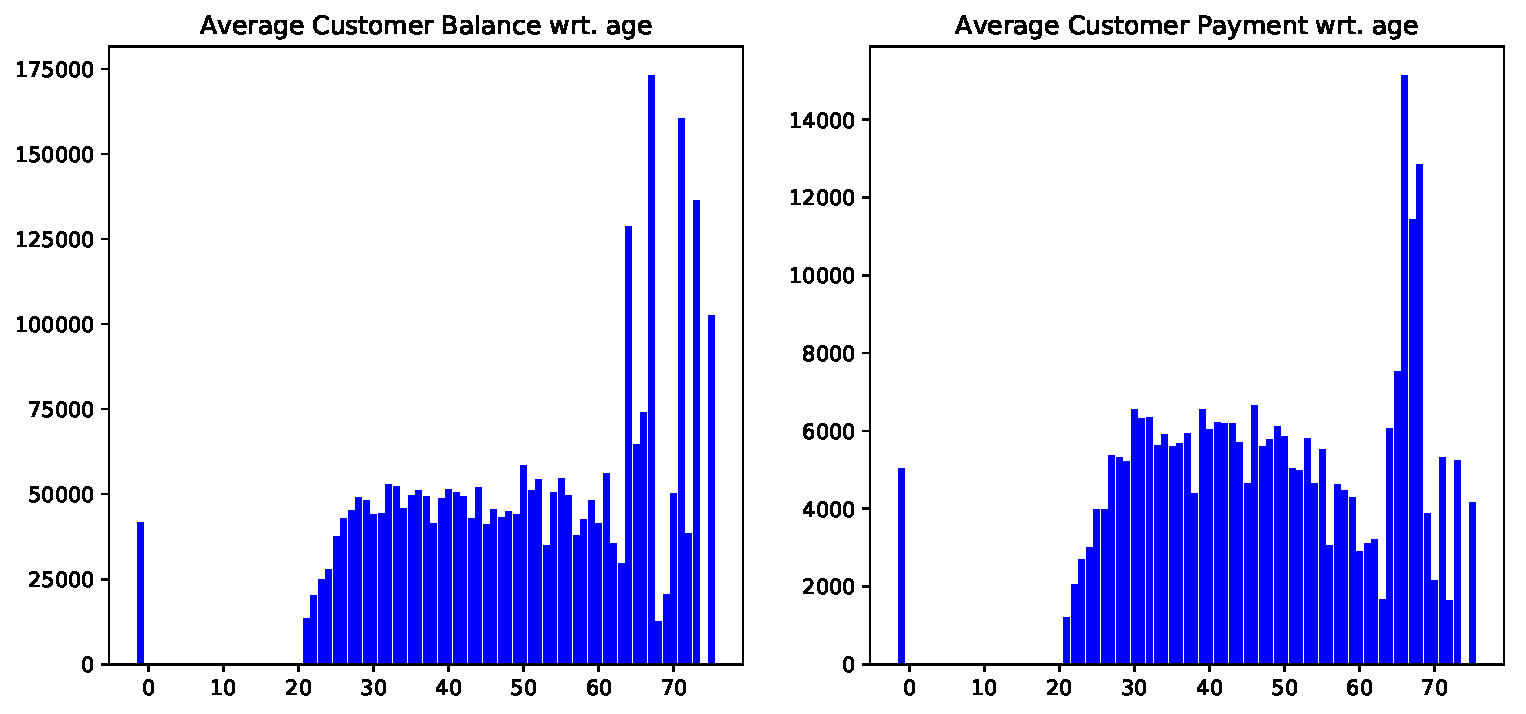
\includegraphics[width=0.9\textwidth]{../Code/Daniele/Plots/age_plot.pdf}
\caption{Plot of the average customer balance and payments over all considered months, in comparison with the age }
\label{average_months}

\end{figure}
\end{center}

\item \textbf{Education}

\todo{Add references supporting "generally"}
Generally, people with a higher education tend to earn more than people with a lower education level and consequently enjoy a higher living standard in Taiwan. As Figure \ref{average_education_ba_pa} shows, this fact reflects on an increased spending and increased balance availability for people that went to graduate school or university wrt. people who just attained a high school certificate. 


\begin{center}
\begin{figure}

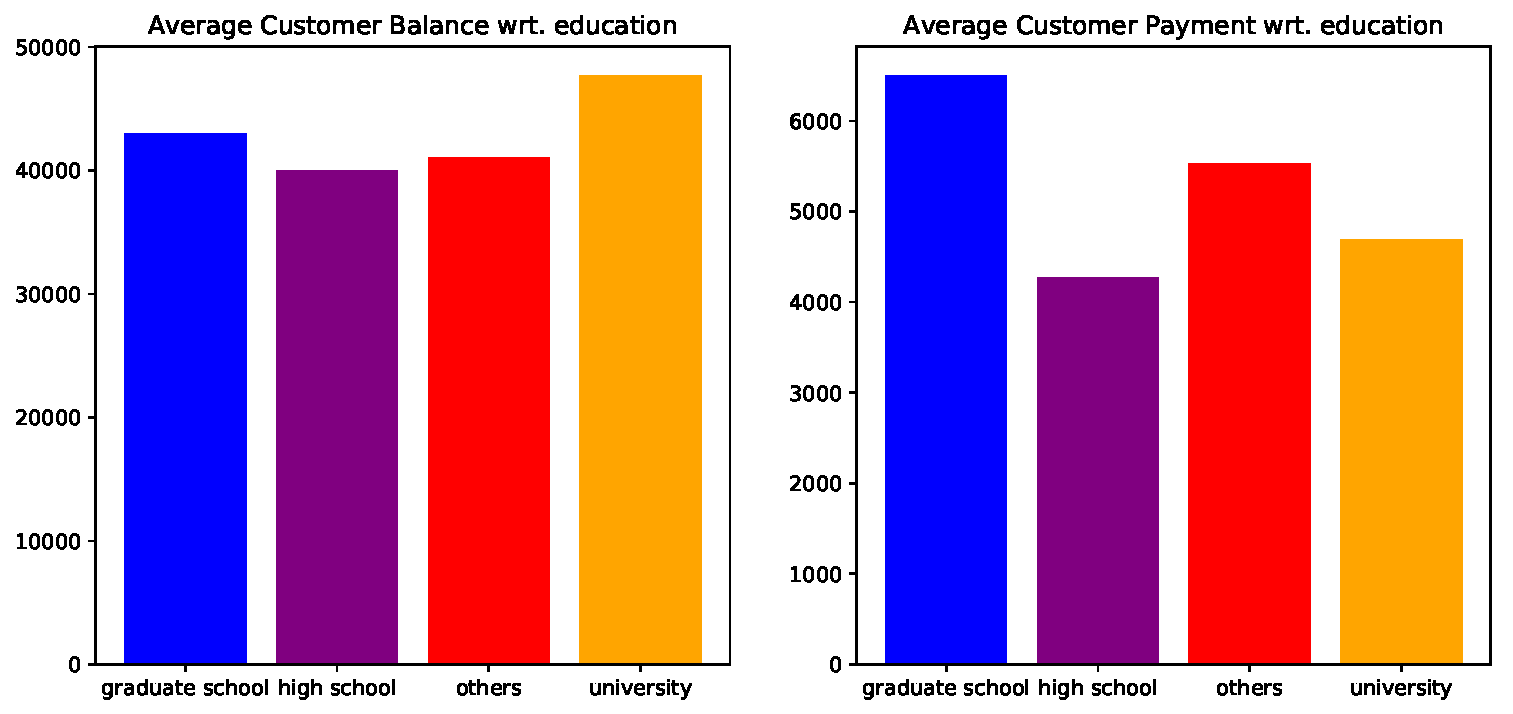
\includegraphics[width=0.9\textwidth]{../Code/Daniele/Plots/education_plot.pdf}
\caption{Plot of the average customer balance and payments over all considered months, in comparison with the education }
\label{average_education_ba_pa}

\end{figure}
\end{center}

\item \textbf{Credit Default}

As by Figure \ref{credit_default_ba_pa}, there seems to be a rather strong correlation between customer payments and a customer default. In fact, the mean value of the average customer payment over all considered months of customers who defaulted is approx. half of the average customer payment over all considered months of customers that did not default. 
We can hence conclude that a low customer revenue is a key factor for understanding whether a customer is going to default. 

On the other hand, the balance doesn't seem to be very strongly correlated with defaults. 

\begin{center}
\begin{figure}

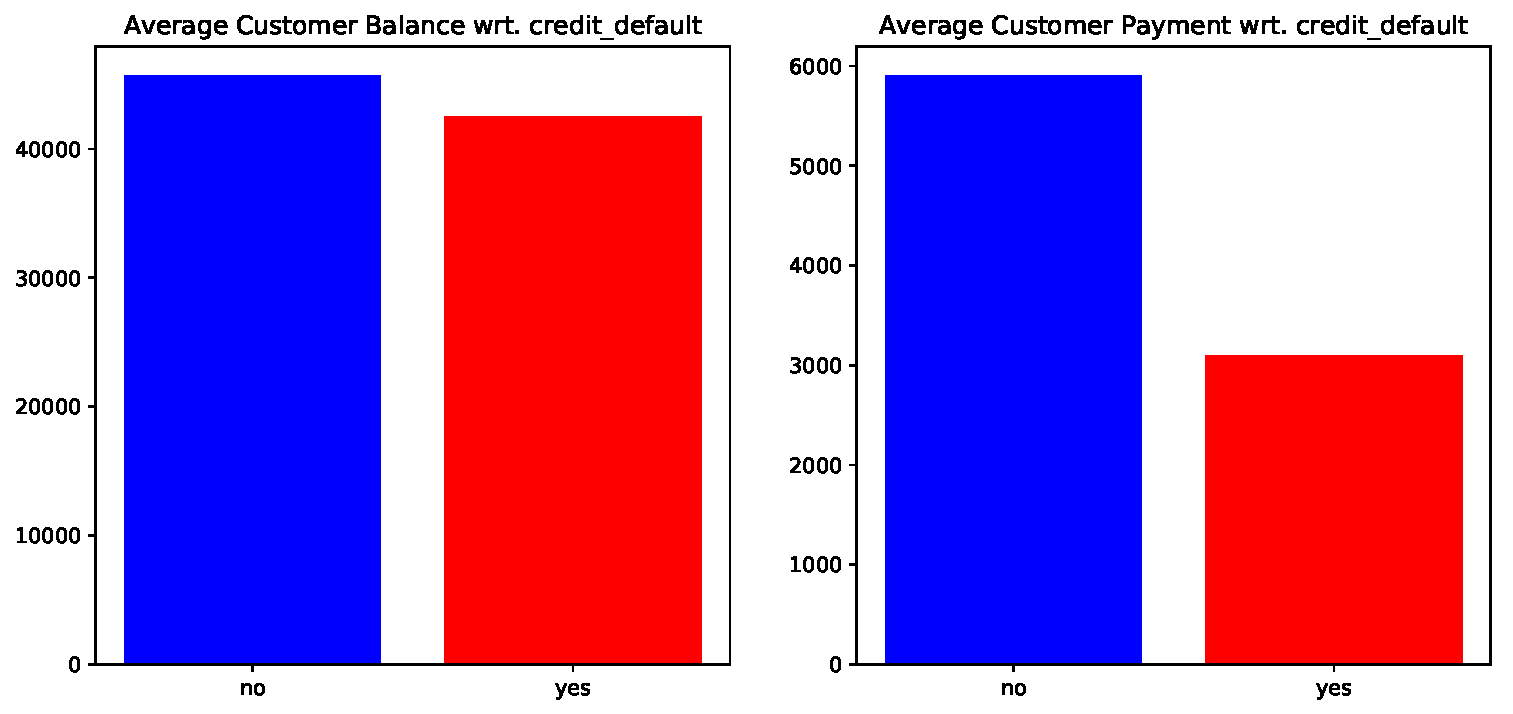
\includegraphics[width=0.9\textwidth]{../Code/Daniele/Plots/credit_default_plot.pdf}
\caption{Plot of the average customer balance and payments over all considered months, in comparison with the education }
\label{credit_default_ba_pa}

\end{figure}
\end{center}

This fact is further highlighted by the scatter plot in Figure \ref{scatter_pa_age}: we can see that defaults occur over all ages, however these typically occur to people with little payments' amounts. Instead, from Figure \ref{scatter_ba_age}, we can see that defaults are not particularly correlated to age or balance. 

\todo{re-generate plots when people with age = 0 have been removed}

\begin{figure}
    \centering
    \begin{subfigure}[b]{0.4\textwidth}
        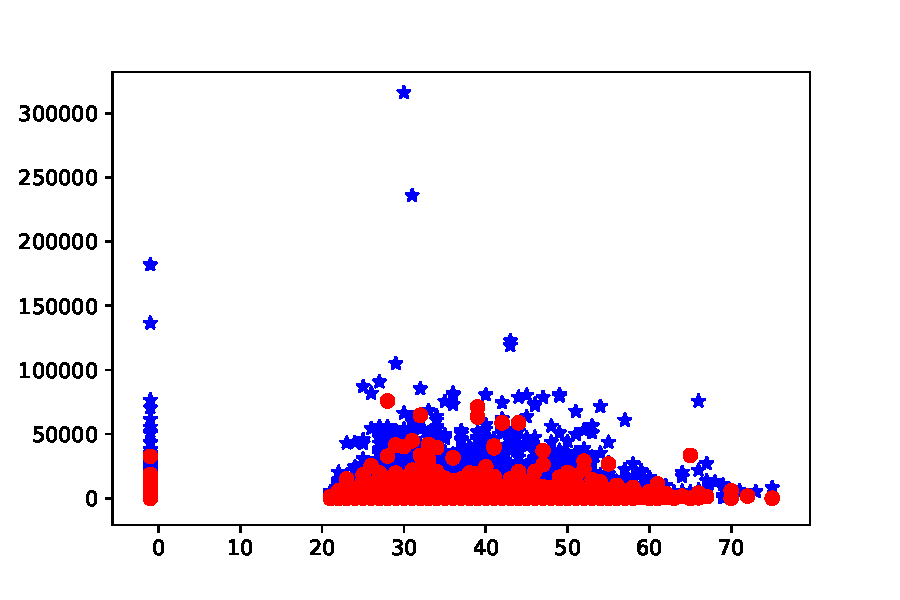
\includegraphics[width=\textwidth]{../Code/Daniele/Plots/scatter_plot_age_pa.pdf}
        \caption{Scatter plot of the average customer payments over all considered months wrt. the age}
        \label{scatter_pa_age}
    \end{subfigure}
    ~ %add desired spacing between images, e. g. ~, \quad, \qquad, \hfill etc. 
      %(or a blank line to force the subfigure onto a new line)
    \begin{subfigure}[b]{0.4\textwidth}
        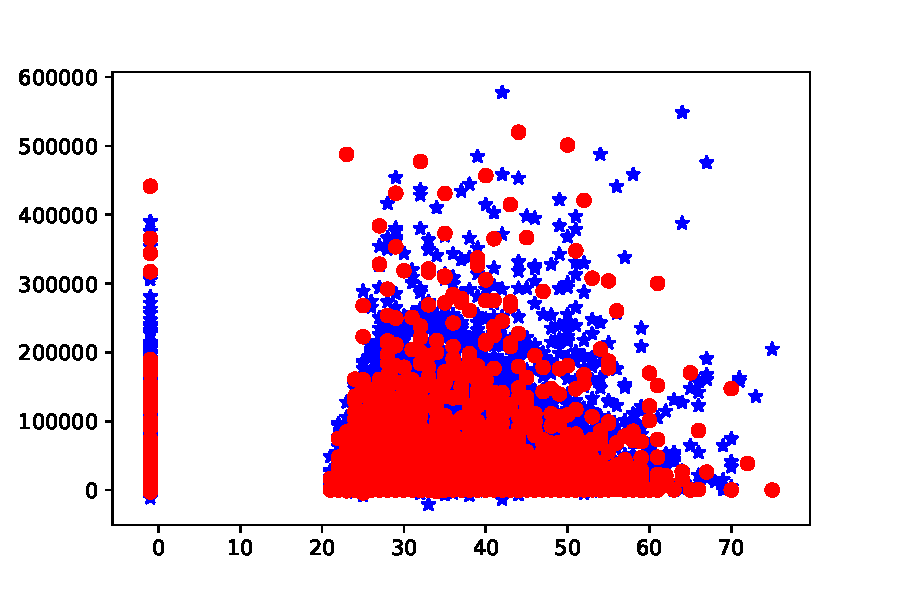
\includegraphics[width=\textwidth]{../Code/Daniele/Plots/scatter_plot_age_ba.pdf}
        \caption{Scatter plot of the average customer balance over all considered months wrt. the age}
        \label{fig:tiger}
    \end{subfigure}
    ~ %add desired spacing between images, e. g. ~, \quad, \qquad, \hfill etc. 
    %(or a blank line to force the subfigure onto a new line)
    \caption{Scatter plots of the customer balance and payments wrt. the age}\label{fig:animals}
\end{figure}


\end{enumerate}


\subsection{Bank Account holders' count}

We now proceed to analyze the count of bank account holders wrt. categorical attributes via bar plots.

\begin{enumerate}
	\item \textbf{Credit Defaults, Status, Gender, Education}
	As it can be seen in Figure \ref{count_default_status_gender_education}, most of the customers did not default. They are similarly distributed among single and married. Most of them are female, and are generally highly educated (university, graduate school). 
	
	The prototypical customer is hence: not defaulted, female, single, university educated. 
	
	
\begin{center}
\begin{figure}

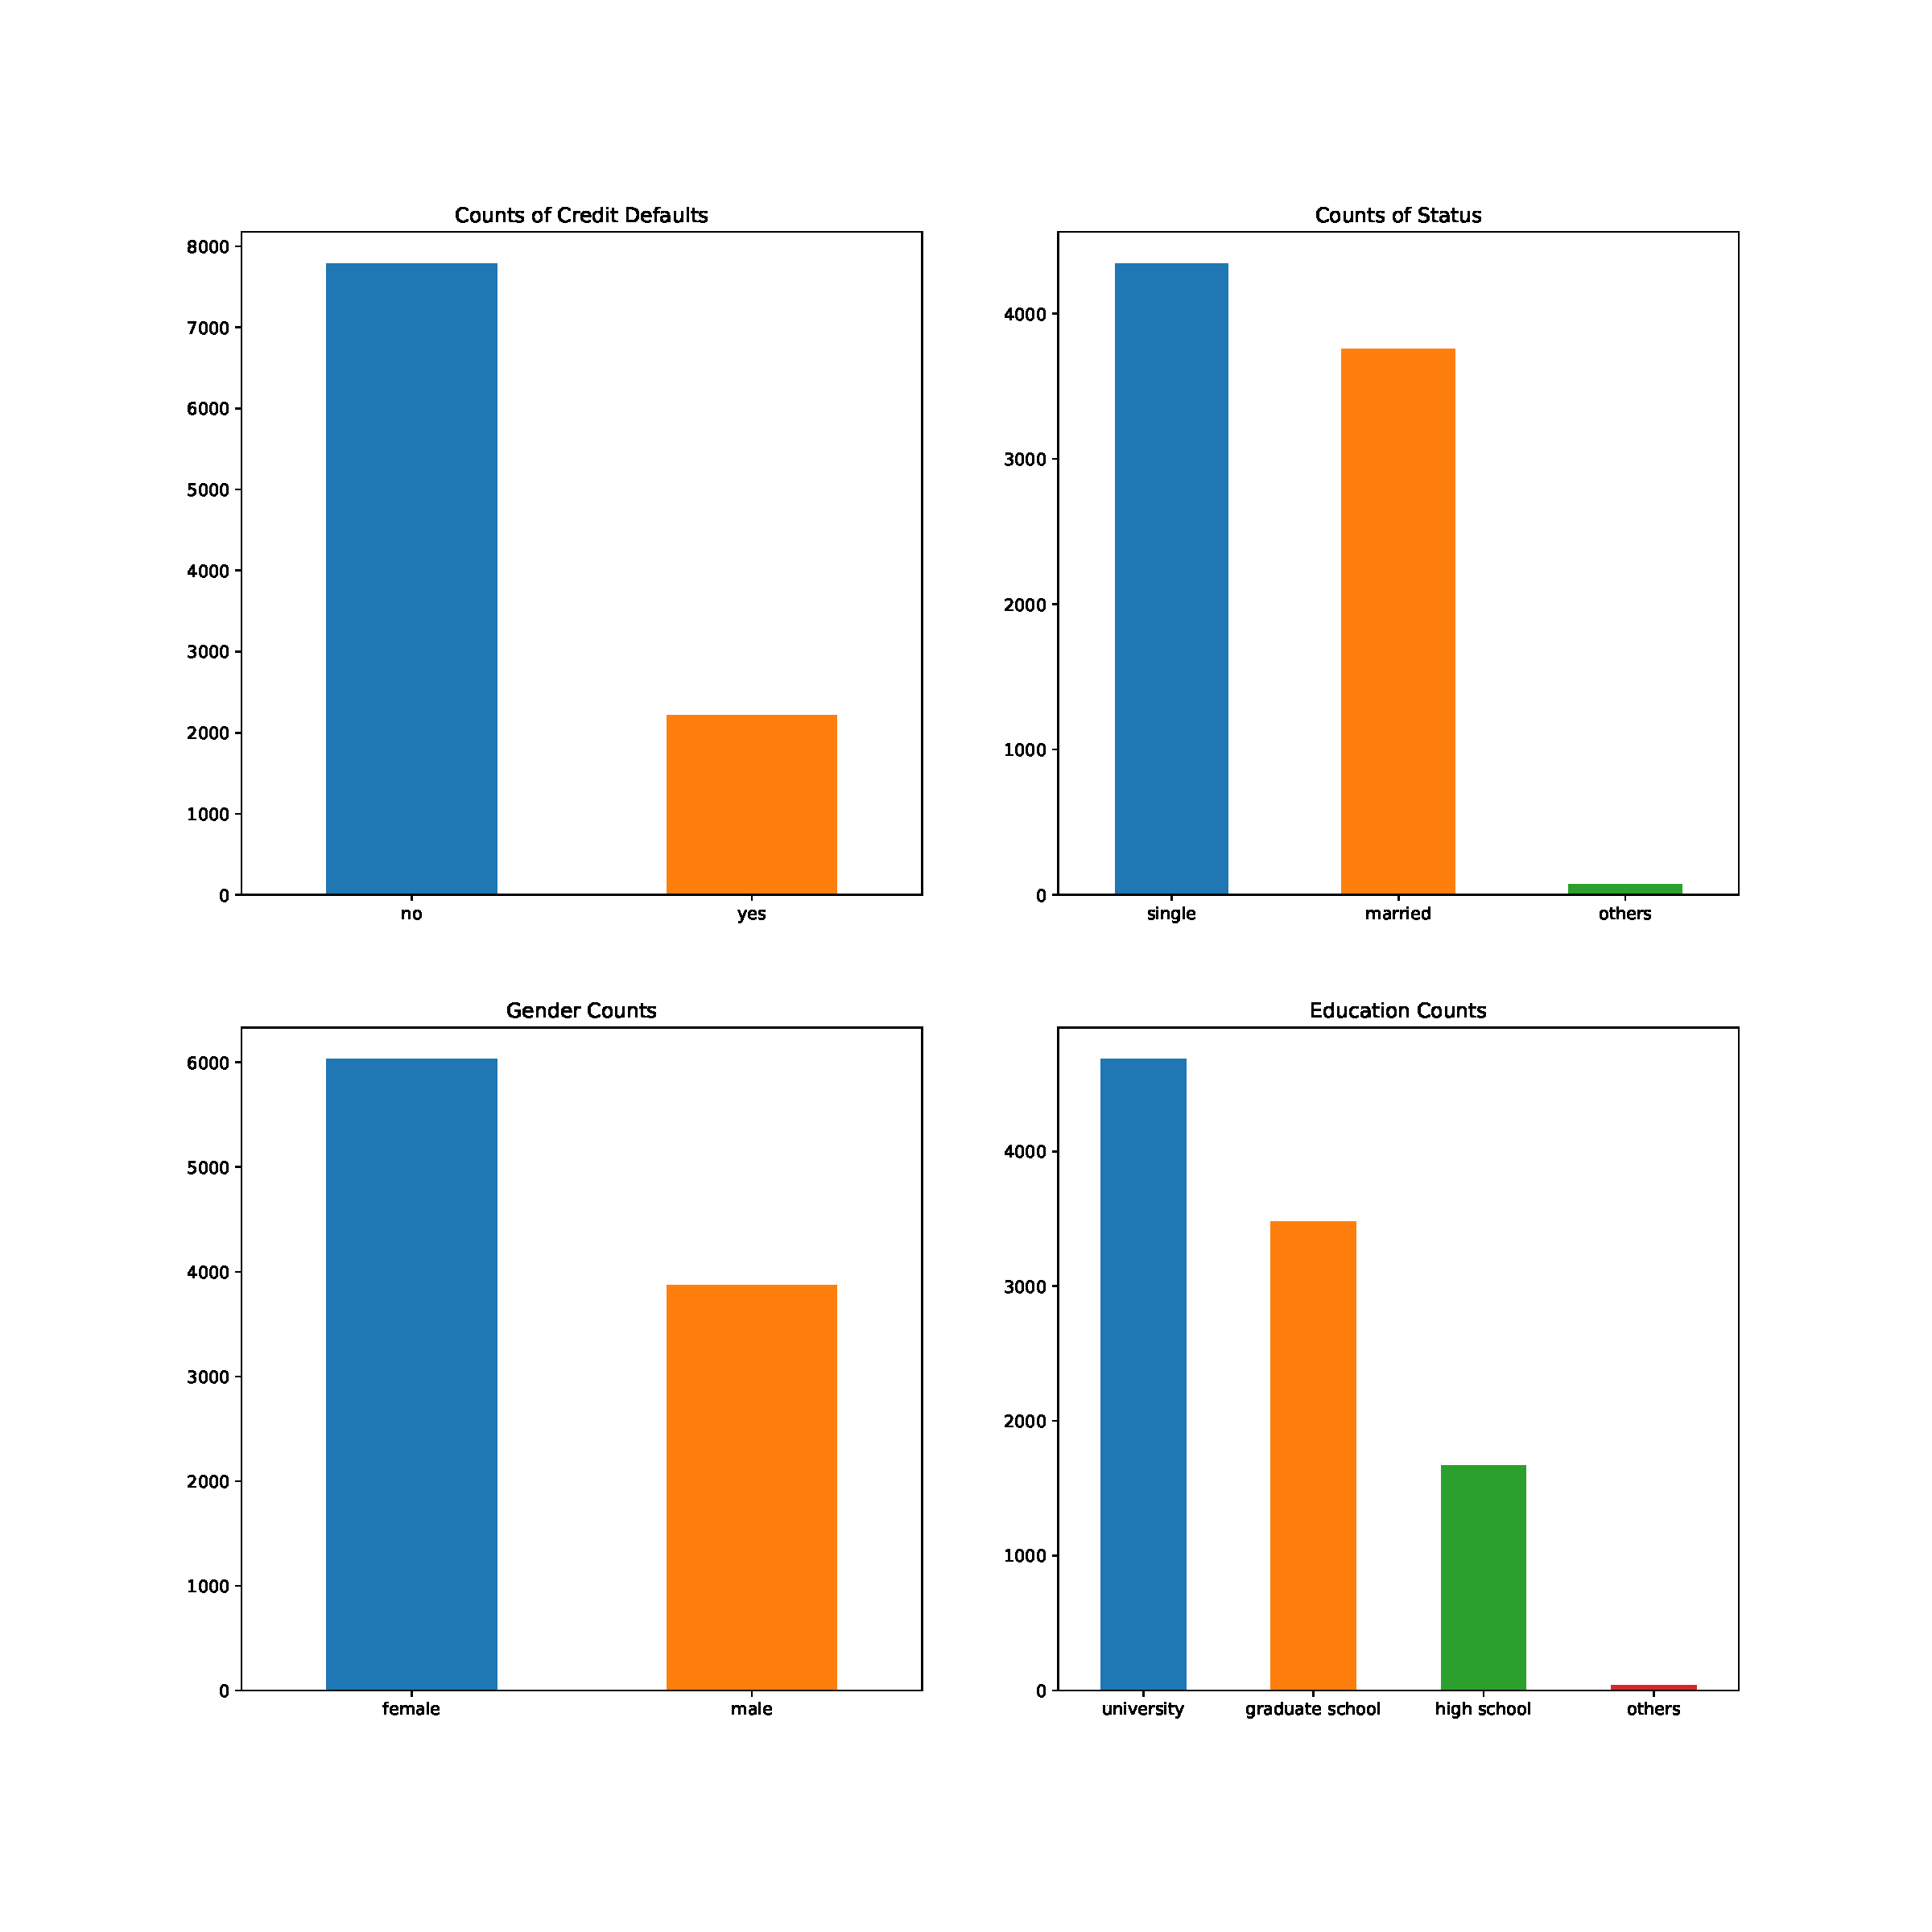
\includegraphics[width=0.9\textwidth]{../Code/Daniele/Plots/counts_plot.pdf}
\caption{Plots of the amount of occurrences for the categories of discrete attributes: credit defaults, status, gender and education }
\label{count_default_status_gender_education}
\end{figure}
\end{center}

And now we analyze the count of bank account holders wrt. continuous attributes via histograms in Figure \ref{hist_continuous_attributes}. We can clearly see that most of the customers are young, and in the range 20-30. The more the age increases, the fewer customers there are. The balance is also mostly up to 100000, and the limit lies in this range. 
\item \textbf{Age, Balance, Expenses, Limit}

\begin{center}
\begin{figure}

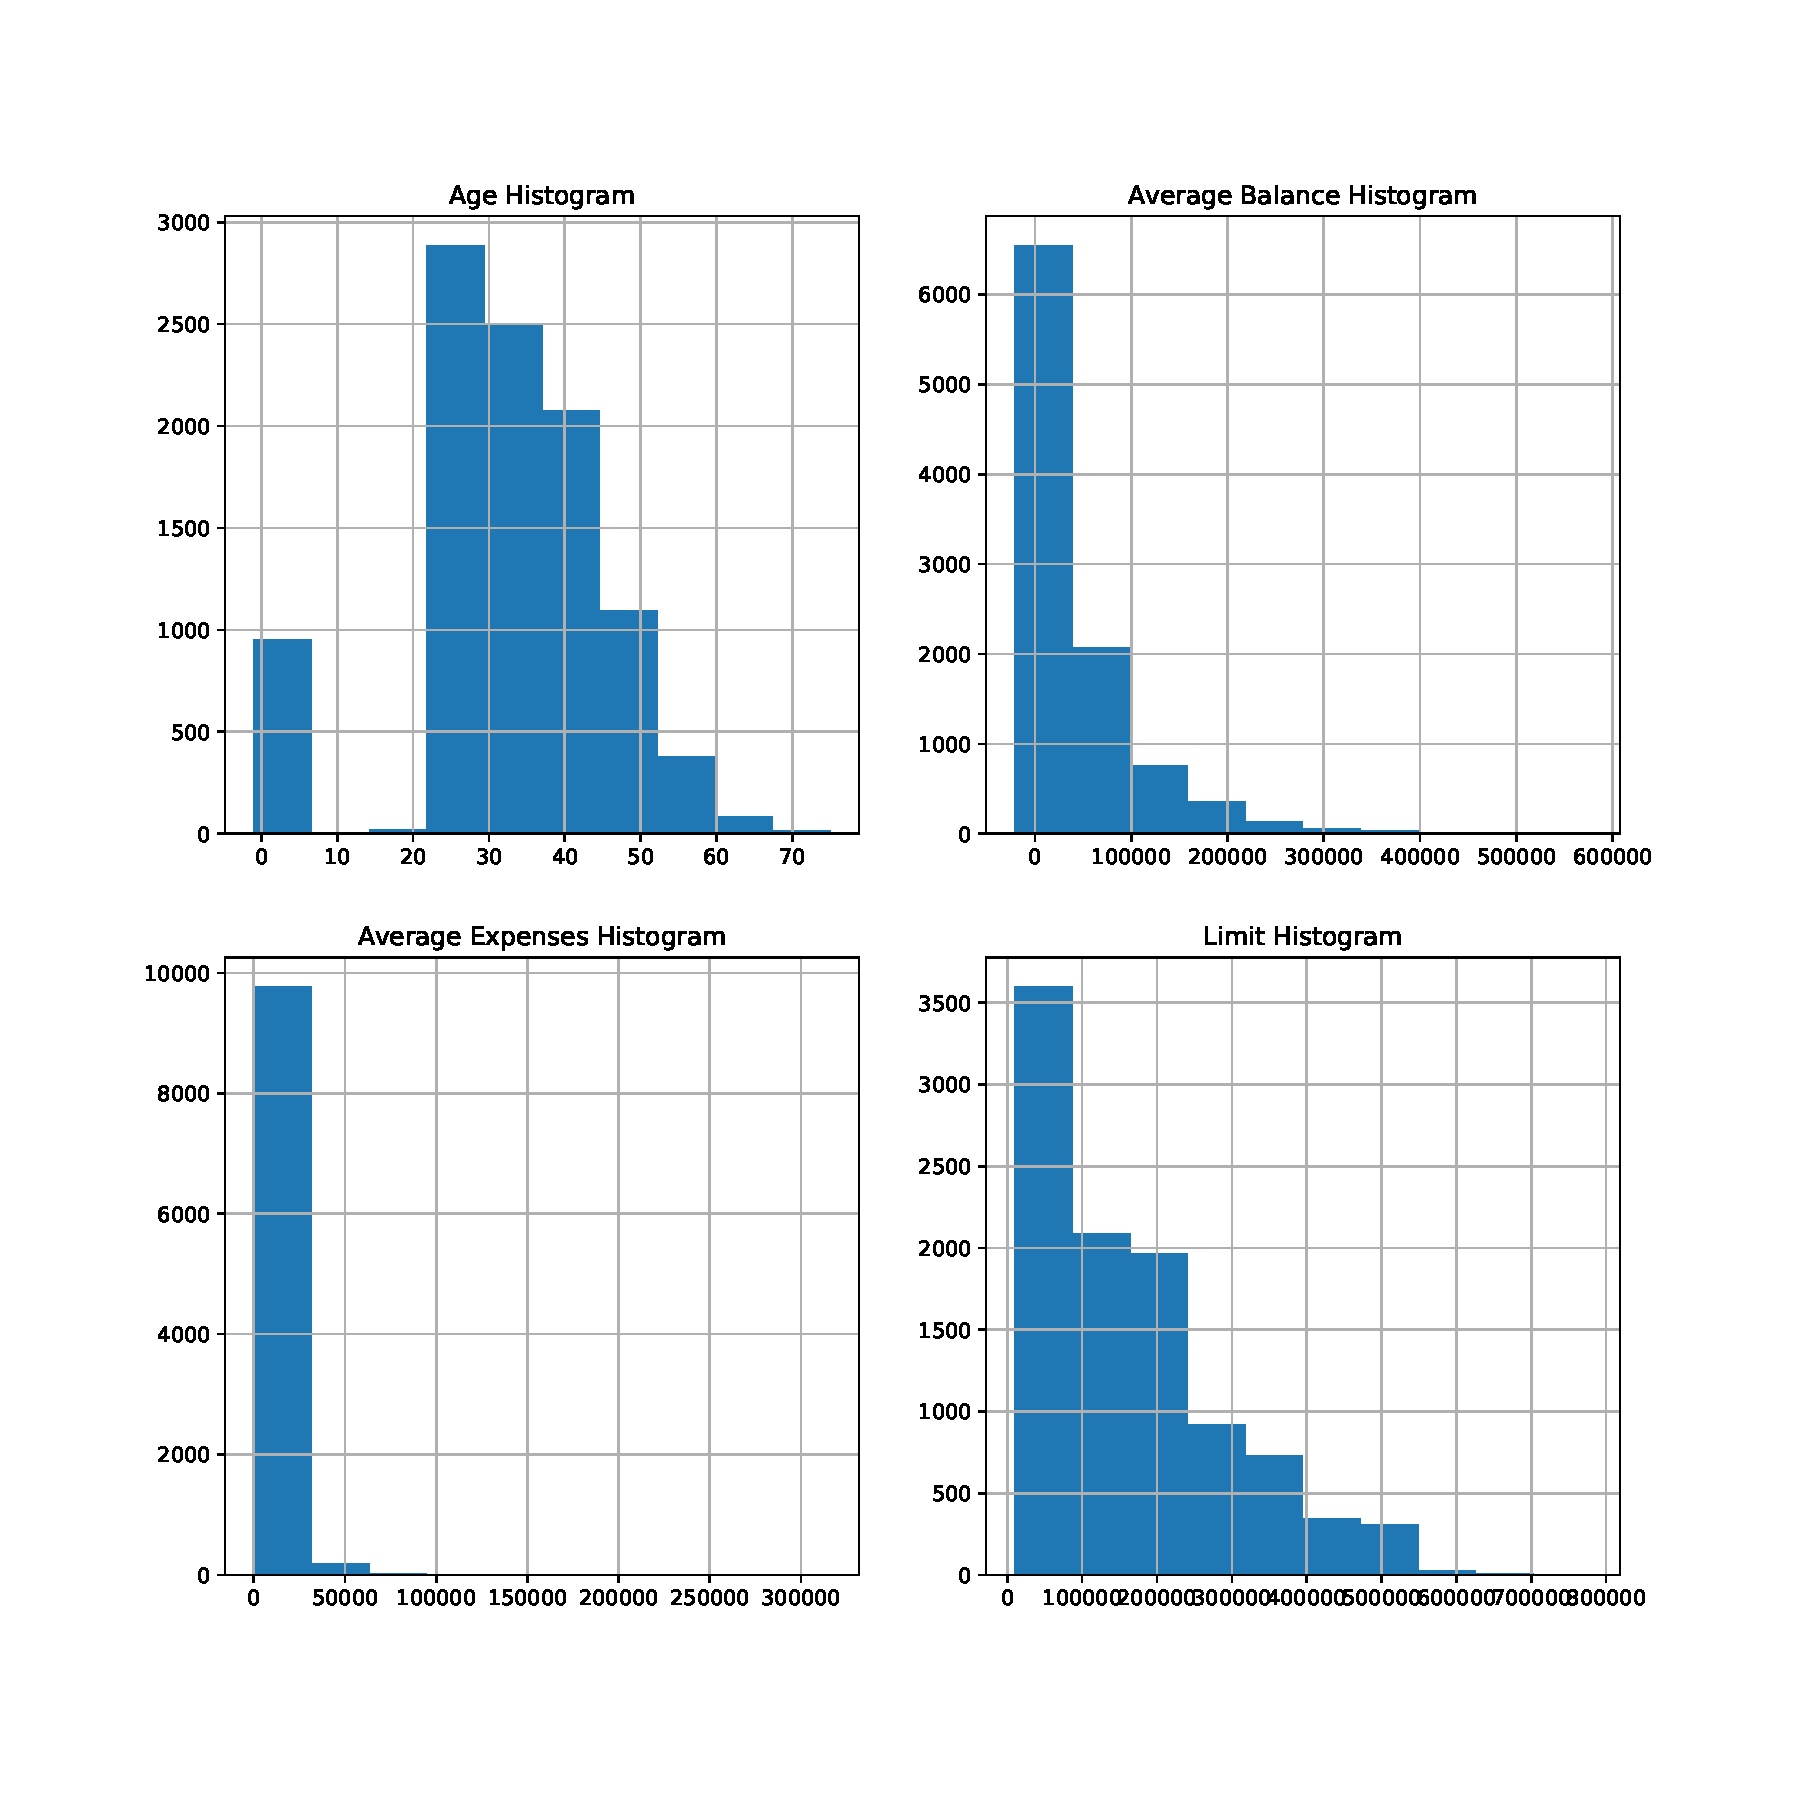
\includegraphics[width=0.9\textwidth]{../Code/Daniele/Plots/age_balance_expenses_limit_hist.pdf}
\caption{Plots of the amount of occurrences for continuous attributes: age, balance, expenses and limit}
\label{hist_continuous_attributes}
\end{figure}
\end{center}
	
\end{enumerate}



\subsection{Credit Default Analysis}

We now proceed to focus our analysis on the relation of the "credit\_default" attribute wrt. different other attributes, in order to understand which correlations leading to a credit default subsist in the data. 

    \begin{figure*}
        \centering
        \begin{subfigure}[b]{0.475\textwidth}
            \centering
            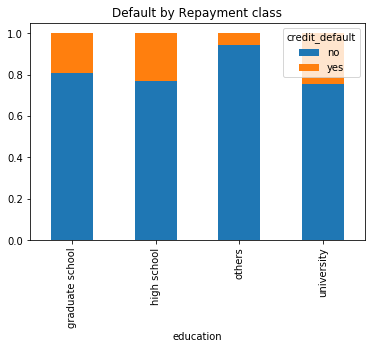
\includegraphics[width=\textwidth]{../Code/Daniele/Plots/credit_default_education.png}
            \caption[Network2]%
            {{\small Network 1}}    
            \label{fig:default_edu}
        \end{subfigure}
        \hfill
        \begin{subfigure}[b]{0.475\textwidth}  
            \centering 
            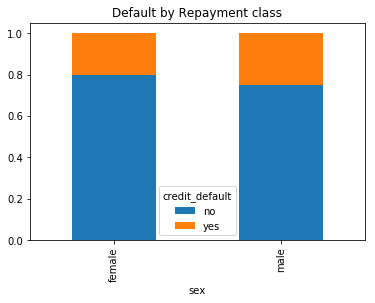
\includegraphics[width=\textwidth]{../Code/Daniele/Plots/credit_default_sex.png}
            \caption[]%
            {{\small Network 2}}    
            \label{fig:default_sex}
        \end{subfigure}
        \vskip\baselineskip
        \begin{subfigure}[b]{0.475\textwidth}   
            \centering 
            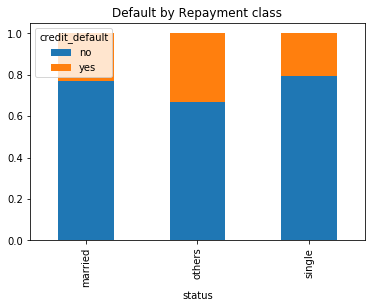
\includegraphics[width=\textwidth]{../Code/Daniele/Plots/credit_default_status_ps.png}
            \caption[]%
            {{\small Network 3}}    
            \label{fig:default_status}
        \end{subfigure}
        \quad
       
        \caption{Default's occurrence wrt. education, sex, status}
        \label{fig:default}
    \end{figure*}
    
    
    In Figure \ref{fig:default_edu}, we can see that bank account holders with an  "others" education appear to be least likely to default than the other categories. 
    From Figure \ref{fig:default_sex}, we see that the gender is not a very significant factor that signalises a possible default, whereas from Figure \ref{fig:default_status}, we recognize that people in the "others" status were more likely to default than married or single people. 
    
    \subsubsection{Ps-analysis}
    
    
    
\begin{center}
\begin{figure}
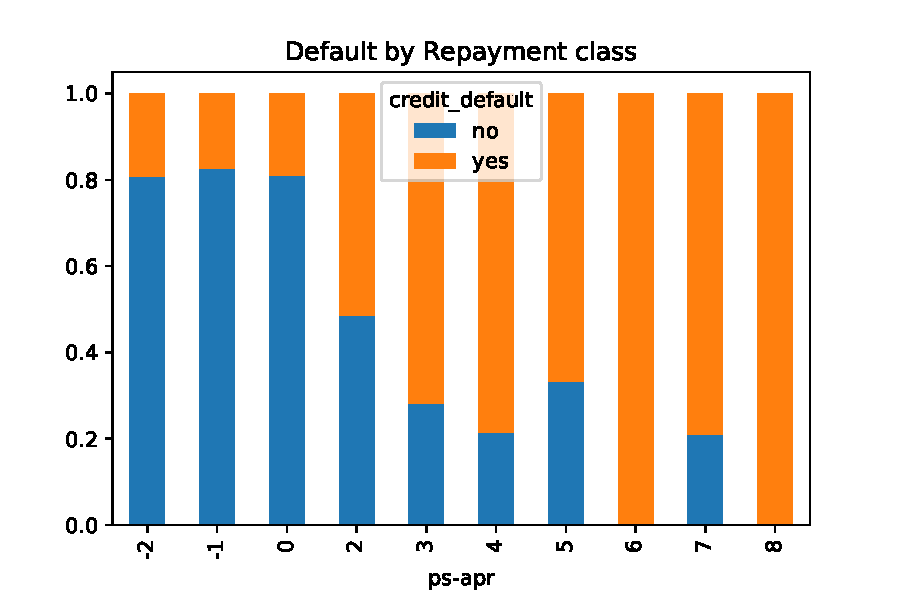
\includegraphics[width=0.9\textwidth]{../Code/Daniele/Plots/credit_default_ps_apr.pdf}
\caption{Plot of the credit\_default occurrence by repayment class (ps)}
\label{fig:repayment_ps_apr}
\end{figure}
\end{center}


From Figure \ref{repayment_ps_apr}, we can see that the higher the ps, the higher is the probability of a default to occur. This behaviour is typical of all the "ps" attributes in the considered dataset. This hence suggests that the "ps" is strongly correlated with the occurrence of a default. 

\section{Syntactic and Semantic Accurance}
The goal of this analysis is to check if all the values of a specific attribute belong to the column domain and if there are typing error.
The following table shows for each attribute its type and all (or in part) its values:

\begin{tabular}{ l | l | l }
\hline
Name & Type & Values\\\hline
limit & int & 10000, 20000,  30000,  40000, \dots,   710000, 740000, 750000, 780000 \\
sex & object & male, female, NaN \\
education  & object & graduate school, university, high school, others, NaN \\
status & object & married, single, others, NaN \\
age & int &  -1, 21, 22, 23, ..., 70, 71, 72, 73, 75 \\
ps-sep & int &  -2, -1,  0,  1,  2,  3,  4,  5,  6,  7,  8 \\
ps-aug & int &  -2, -1,  0,  1,  2,  3,  4,  5,  6,  7 \\
ps-jul & int &  -2, -1,  0, 1,  2,  3,  4,  5,  6,  7,  8 \\
ps-jun & int &  -2, -1,  0,  2,  3,  4,  5,  6,  7,  8 \\
ps-may & int &  -2, -1,  0,  2,  3,  4,  5,  6,  7,  8 \\
ps-apr  & int &  -2, -1,  0,  2,  3,  4,  5,  6,  7,  8 \\
ba-sep & int &  -14386, -10682,  -9802,  ... , 588000, 604019, 613860 \\
ba-aug & int &  -69777, -67526, -30000, ... , 577681, 597793, 605943 \\
ba-jul & int &  -61506, -24702, -15910, ... , 577015, 578971, 597415 \\
ba-jun & int &  -24303, -15910, -15588, ... , 565669, 569034, 616836 \\
ba-may & int &  -81334, -61372, -37594, ... , 530672, 551702, 587067 \\
ba-apr & int &  -209051, -150953,  -57060, ... ,  478034,  527566,  568638 \\
pa-sep & int &   0, 1, 2, ... , 304815, 323014, 493358 \\
pa-aug & int &   0, 1, 2, ... , 401003,  580464, 1227082 \\
pa-jul & int &   0, 1, 2, ... , 349395, 400972, 417588 \\
pa-jun & int &   0, 1, 2, ... , 291227, 292462, 292962 \\
pa-may & int &  0, 1, 2, ... , 303512, 331788, 417990 \\
pa-apr & int &   0, 1, 2 , ... , 403500, 443001, 528666 \\
credit\_defaut & object &  yes, no \\
\hline
\end{tabular}\bigskip\\	
From this table it's possible to notice the following problems:
\begin{enumerate}
\item The attributes 'Sex', 'Education' and 'Status' have a wrong value: Not a Number;
\item The attribute 'Age' has a wrong value that is '-1'.
\end{enumerate}
All others attribute are semantically and syntactically correct!

	
    
    
    













\bibliographystyle{plain}
\bibliography{bibtex}

\end{document}
              
